\documentclass[10pt, aspectratio=169]{beamer}

\usepackage{tgschola}
\usepackage{subfig}
\usepackage{float}
\usepackage{wrapfig}

\title{Brain Tumor Detection using Machine Learning Models}

\subtitle{B.Sc. Semester VI Project \newline Department of Computer Science, Gurudas College}

\usetheme{Madrid}

\date{}

\author[Rajarshi, Bhargav, Soptorshi, Brahmajit] {
	Bhargav Basu \texorpdfstring{\\} \and
	Soptorshi Bhattacharjee \texorpdfstring{\\} \and
	Brahmajit Das \texorpdfstring{\\} \and
	Rajarshi Sardar
}

\institute[Gurudas College]{Gurudas College, Calcutta University}

\begin{document}

	\begin{frame}
		\titlepage
	\end{frame}

	\begin{frame}
		\frametitle{Overview}
		\begin{columns}[totalwidth=0.9\textwidth]
			\hspace*{2.5cm}
			\begin{column}{0.35\textwidth}
				\tableofcontents[sections={1-4}]
			\end{column}
			\begin{column}{0.35\textwidth}
				\tableofcontents[sections={5-9}]
			\end{column}
		\end{columns}
	\end{frame}

	\section{Motivation}
	\begin{frame}
		\frametitle{Motivation}

		The motivation is to develop a software with better segmentation
		capability for use in medical imaging to detect diseases like brain
		tumor. Image segmentation has been identified as the key problem of
		medical image analysis and remains a popular and challenging area of
		research. Image segmentation is increasingly used in many clinical and
		research applications to analyze medical imaging datasets; which
		motivated us to present a snapshot of dynamically changing field of
		medical image segmentation.

		\vspace{0.5cm}

		The motivation of this work is to increase patient safety by providing
		better and more precise data for medical decision.
	\end{frame}

	\section{Domain Description}

	\begin{frame}
		\frametitle{Domain Description}

		\begin{itemize}
			\item
			\textbf{Neurological Examination}: It is a series of test to measures
			the function of the patients nervous system and also his/her physical
			and mental alertness. \pause
			\item
			\textbf{Machine Learning}: Machine learning approaches address these
			problems by mainly using hand-crafted features (or pre-defined
			features). \pause
		   \item
		   \textbf{Brain Scans}: Brain scan is a picture of the internal
		   structure of the brain. A specialized machine takes a scan in the
		   same way as a digital camera takes a photograph.
		\end{itemize}
	\end{frame}

	\section{Background}

	\begin{frame}
		\frametitle{Background}

		We propose the use of ML algorithms to overcome the drawbacks of
		traditional classifiers. We investigate and compare the performance of
		various machine learning models, namely \textbf{CNN}, \textbf{VGG 16}
		and \textbf{ ResNet 50 }; implemented using the frameworks Tensorflow
		and fast.ai.
	\end{frame}

	\section{Methodology}

	\begin{frame}
		\frametitle{Methodology}

		\vspace{-1cm}

		\begin{figure}[h]
			\centering
			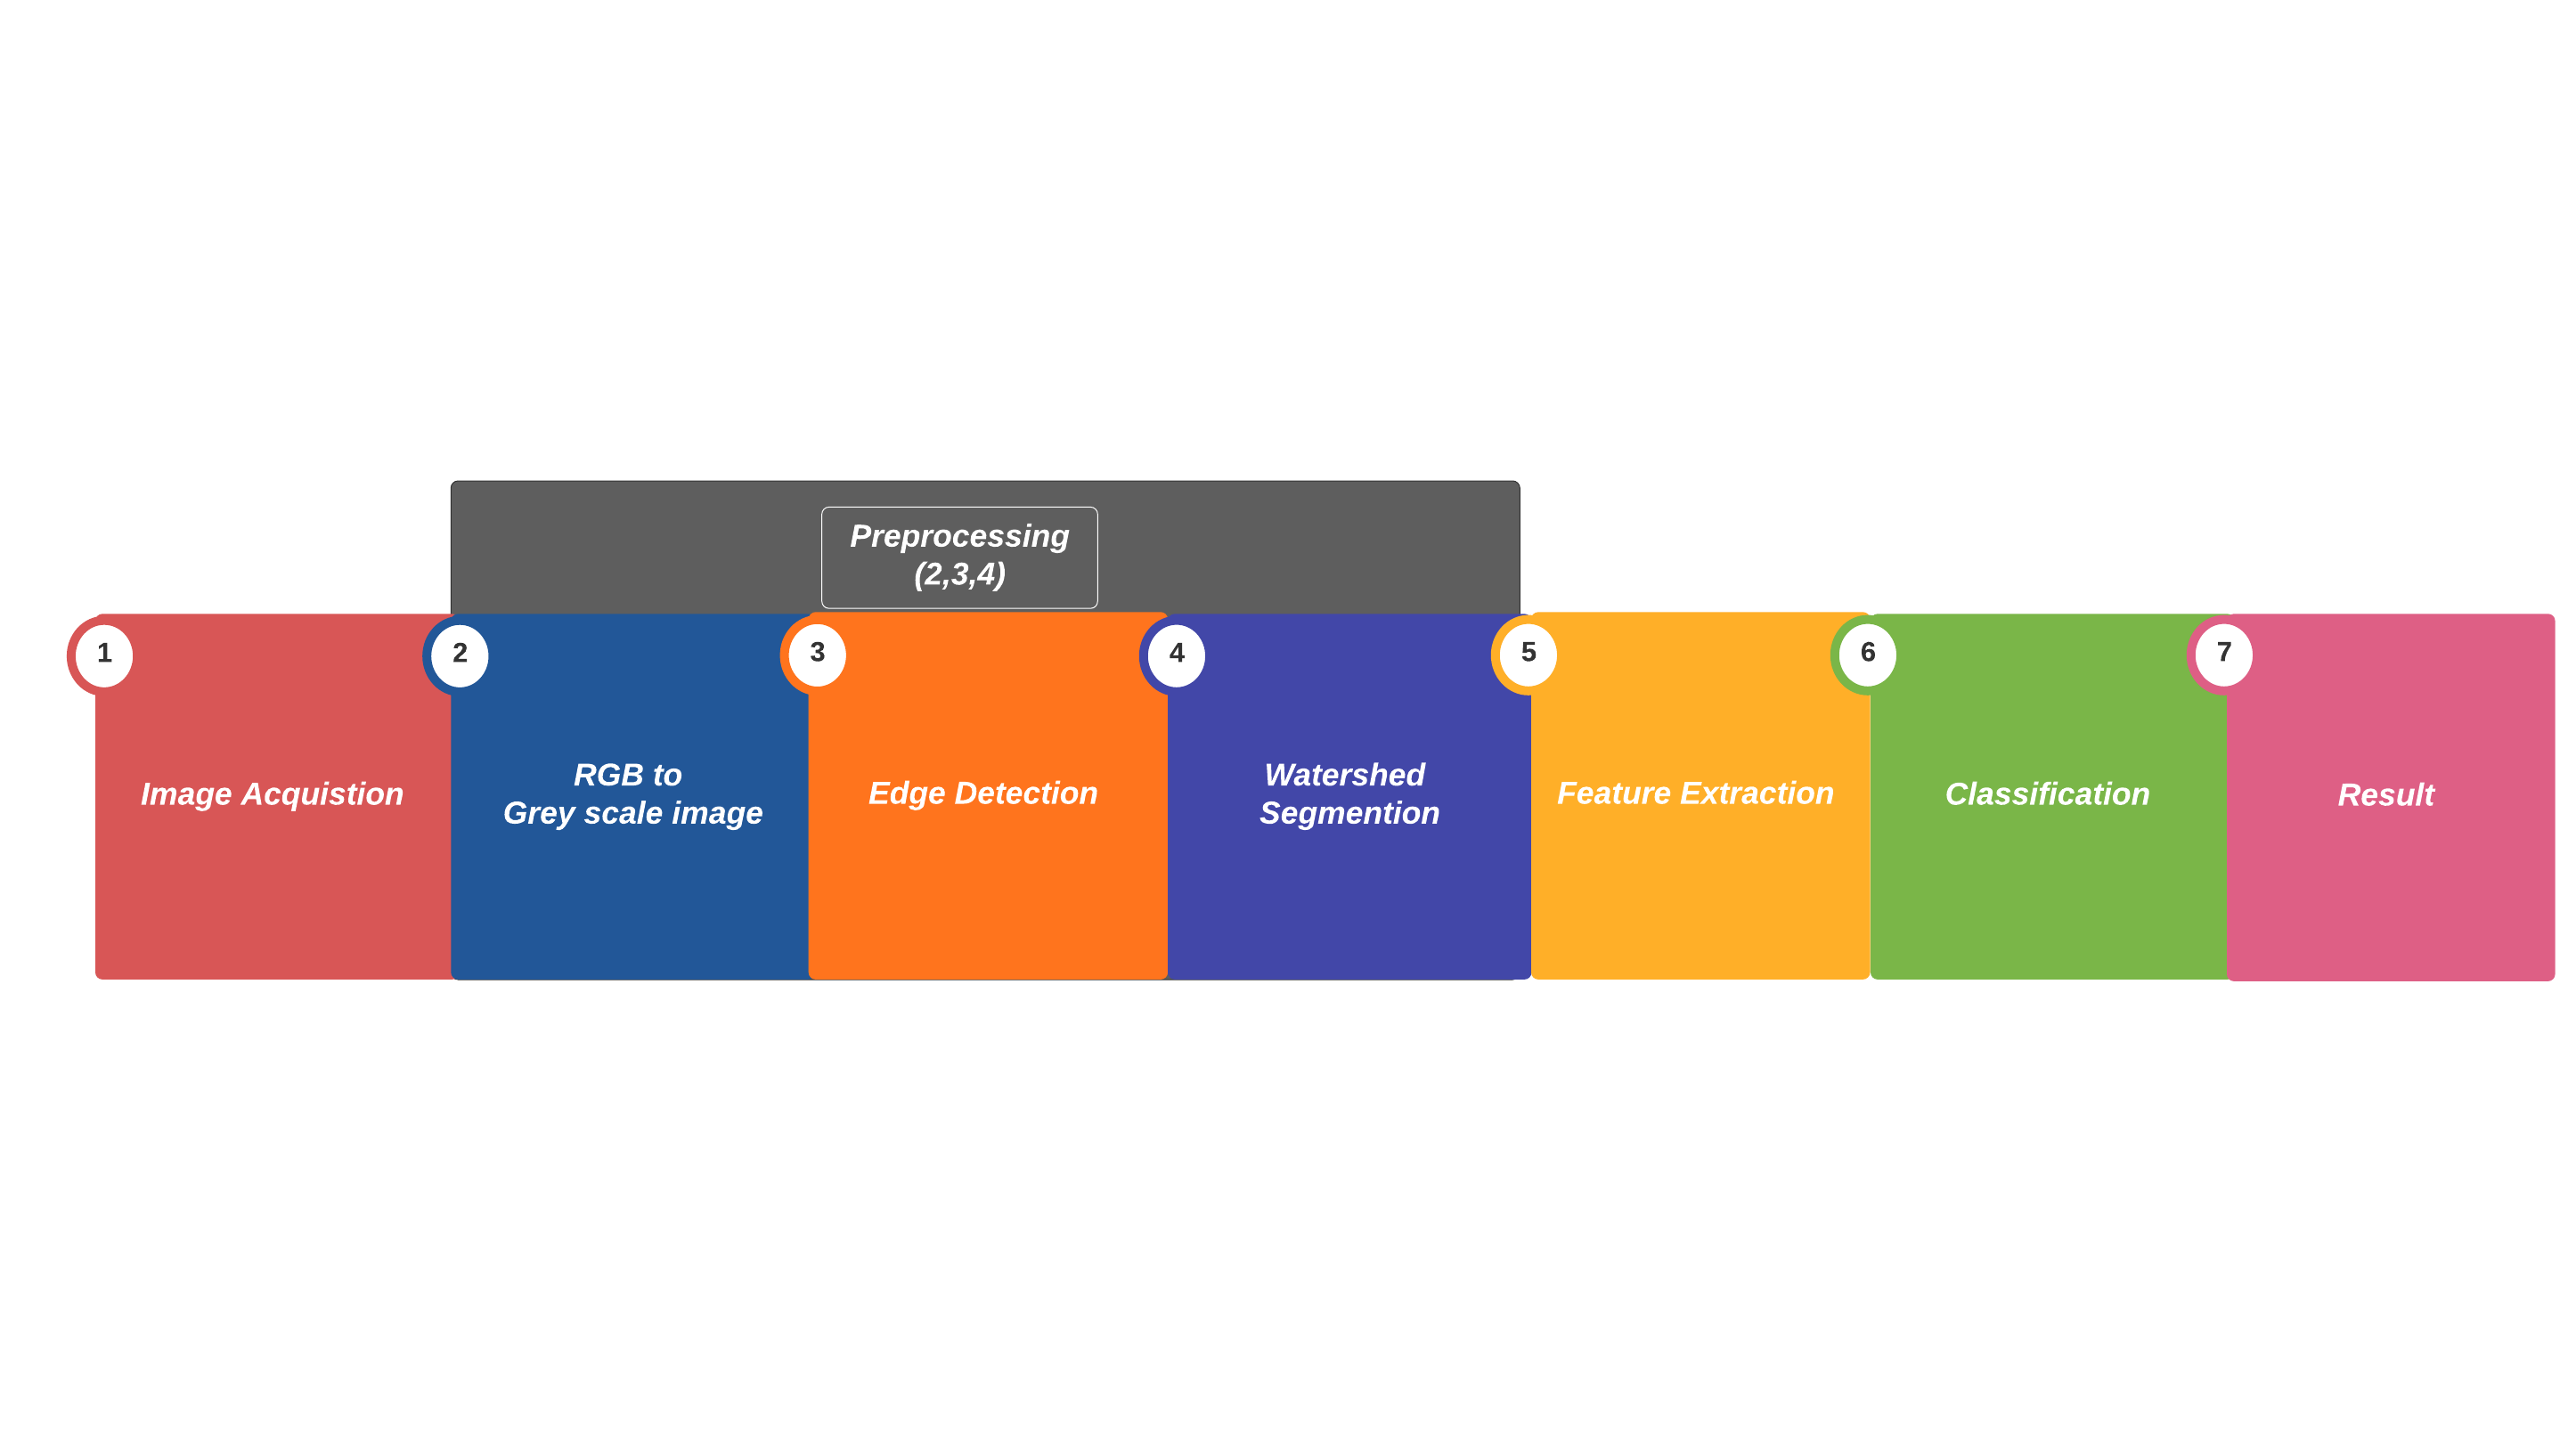
\includegraphics[width=\textwidth]{imgs/flowchart}
			\caption{Proposed Methodology}%
			\label{fig:prop_methodology}
		\end{figure}

	\end{frame}

	\subsection{Image Acquisition}

	\begin{frame}
		\frametitle{Methodology}
		\framesubtitle{Image Acquisition}
		The MRI brain images are acquired and are given as input to
		pre-processing stage.

		\begin{figure}[H]
			\centering
			\subfloat[MRI scan shown no presence of tumor]
			{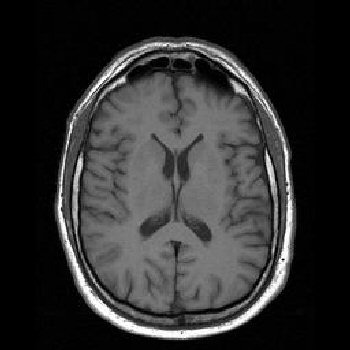
\includegraphics[width=0.25\textwidth]
			{imgs/pred1.jpg}\label{scan2}}
			\hspace{0.2cm}
			\subfloat[MRI scan of a tumorous cell]
			{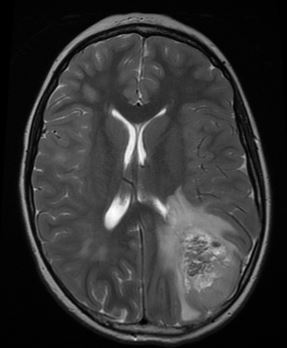
\includegraphics[width=0.2\textwidth]
			{imgs/Y100.JPG}\label{scan1}}
			\caption{MRI Scans}
			\label{MRIScans}
		\end{figure}
	\end{frame}

	\subsection{Preprocessing}

	\begin{frame}
		\frametitle{Methodology}
		\framesubtitle{Preprocessing}

		Preprocessing is needed as it provides improvement in image data which
		enhances some of the image features which are important for further
		processing.

		\vspace{0.5cm}

		Preprocessing includes:

		\begin{itemize}
			\item Binarization
			\item Filtering
			\item Edge Detection
			\item Segmentation
		\end{itemize}

		\begin{block}{Segmentation}
			Image segmentation is the process of partitioning a digital image into multiple
			segments (sets of pixels, also known as image objects). The goal of
			segmentation is to simplify and/or change the representation of an image into
			something that is more meaningful and easier to analyze.
		\end{block}

	\end{frame}

	\begin{frame}
		\begin{figure}[ht]
			\centering
			\subfloat[Original Image]
			{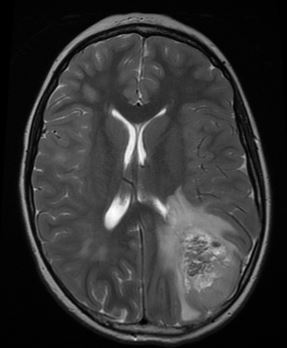
\includegraphics[width=0.2\linewidth]
			{imgs/Y100.JPG}\label{original}}
			\hspace{0.5cm}
			\subfloat[Filtered Imaage]
			{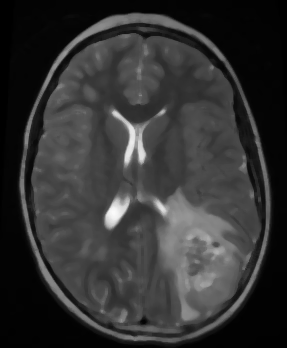
\includegraphics[width=0.2\linewidth]
			{imgs/median_filtering.png}\label{smooted image}}
			\hspace{0.5cm}
			\subfloat[Edge Detection]
			{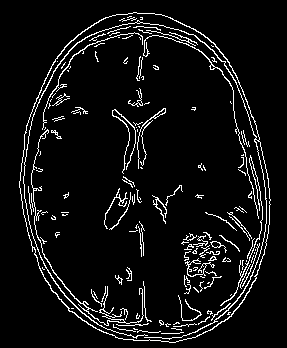
\includegraphics[width=0.2\linewidth]
			{imgs/edges_detection.png}\label{edge detection}}
			\hspace{0.5cm}
			\subfloat[Segmentation]
			{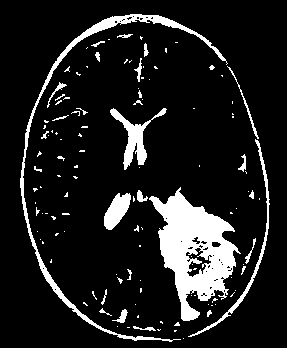
\includegraphics[width=0.2\linewidth]
			{imgs/segmentation.png}\label{segmentation}}
			\caption{preprocessing operations}
			\label{Preprocessing Operations}
		\end{figure}
	\end{frame}

	\subsection{Feature Extraction}

	\begin{frame}
		\frametitle{Methodology}
		\framesubtitle{Feature Extraction}

		When input to an algorithm is very large and redundant to be processed,
		it is transformed into reduced representative set of features called
		feature vector.

		\vspace{1cm}

		These features are extracted using Gray Level Co-occurrence Matrix
		(GLCM) as it is robust method with high performance.
	\end{frame}

	\subsection{Classification}

	\begin{frame}
		\frametitle{Methodology}
		\framesubtitle{Classification}

		The Machine learning algorithms are used for classification of MR brain
		image either as normal or abnormal.  The major aim of ML algorithms is
		to automatically learn and make intelligent decisions.

		\vspace{0.5cm}

		For classification we are using \textbf{CNN}, \textbf{VGG 16} and
		\textbf{ResNet 50}.

		\vspace{0.5cm}

		For this project we are using binary classification, two classes one for
		normal and another for abnormal.

	\end{frame}

	\section{Deep learning}

	\begin{frame}
		\frametitle{Deep Learning}
		\framesubtitle{Why deep learning?}

		\begin{block}{Image Classification}
			Image classification is where a computer can analyze an image and
			identify the ‘class’ the image falls under.
		\end{block}

		\begin{block}{What is deep learning?}
			Deep learning is a type of machine learning; a subset of artificial
			intelligence (AI) that allows machines to learn from data. Deep
			learning involves the use of computer systems known as neural
			networks.
		\end{block}

		\begin{block}{Why use deep learning for image classification}
			Deep learning allows machines to identify and extract features from
			images. This means they can learn the features to look for in images
			by analysing lots of pictures. So, programmers don’t need to enter
			these filters by hand.
		\end{block}

	\end{frame}

	\section{Models}

	\begin{frame}
		\frametitle{Model}
		\framesubtitle{CNN}


		CNN or Convolutional Neural Network a class of artificial neural
		network, most commonly applied to analyze visual imagery.They are also
		known as shift invariant or space invariant artificial neural networks
		(SIANN), based on the shared-weight architecture of the convolution
		kernels or filters that slide along input features and provide
		translation equivariant responses known as feature maps.

	\end{frame}

	\begin{frame}
		\begin{figure}[h]
			\centering
			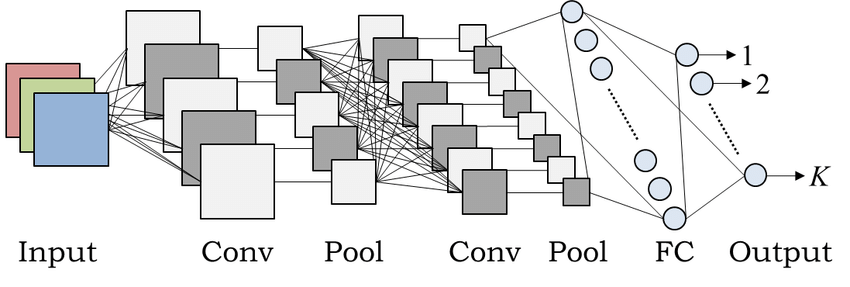
\includegraphics[width=\linewidth]{imgs/cnn_arch.png}
			\caption{CNN's architecture}%
			\label{fig:imgs/cnn_arch}
		\end{figure}
	\end{frame}

	\begin{frame}
		\frametitle{Model}
		\framesubtitle{VGG 16}

		VGG 16 is is a significantly more accurate ConvNet architecture, which
		not only achieve state-of-the-art accuracy on ILSVRC classification and
		localisation tasks, but are also applicable to other image recognition
		datasets, where they achieve excellent performance even when used as a
		part of a relatively simple pipelines (e.g. deep features classified by
		a linear SVM without fine-tuning).
	\end{frame}

	\begin{frame}
		\begin{figure}[h]
			\centering
			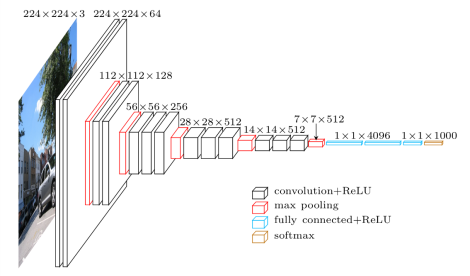
\includegraphics[width=0.8\linewidth]{imgs/vgg16_arch.png}
			\caption{VGG 16's architecture}%
			\label{fig:imgs/vgg16_arch}
		\end{figure}
	\end{frame}

	\begin{frame}
		\frametitle{Model}
		\framesubtitle{ResNet 50}

		ResNet50 is a variant of ResNet model which has 48 Convolution layers
		along with 1 MaxPool and 1 Average Pool layer. It has $3.8 x 10^9$
		Floating points operations. It is a widely used ResNet model and we have
		explored ResNet50 architecture in depth.
	\end{frame}

	\begin{frame}
		\begin{figure}[h]
			\centering
			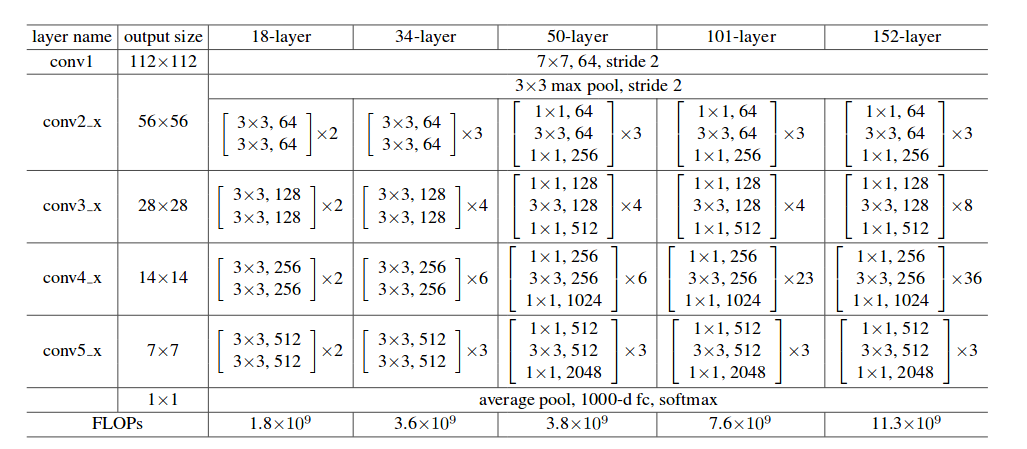
\includegraphics[width=\linewidth]{imgs/resnet_arch.png}
			\caption{Reset's architecture}%
			\label{fig:imgs/resnet_arch2}
		\end{figure}
	\end{frame}

	\section{Implementation}

	\begin{frame}
		\frametitle{Implementation}
		\framesubtitle{Assumptions}

		It is assumed that the MRI scans are collected and processed before
		feeding into the module.

		\vspace{1cm}

		The program is dependent on external modules and are expected to be
		pre-installed on the system. The modules namely include:

		\vspace{1cm}

		\begin{itemize}
			\item Tensorflow
			\item fast.ai
			\item OpenCV
			\item matplotlib
		\end{itemize}
	\end{frame}

	\begin{frame}
		\frametitle{Implementation}
		\framesubtitle{Implementing}

		\begin{itemize}
			\item Acquire Data (MRI Scans)
			\item Dividing the data into two classes while keeping the separate
				batch for prediction
			\item Build the models using the aforementioned libraries
			\item Train the model (feed data into the model)
			\item Evaluate the trained model on the prediction batch
		\end{itemize}
	\end{frame}

	\section{Result}

	\begin{frame}
		\frametitle{Results}
		\framesubtitle{CNN implemented using fast.ai and tensorflow}
		\begin{figure}[H]
			\centering
			\subfloat[cnn using tensorflow]
			{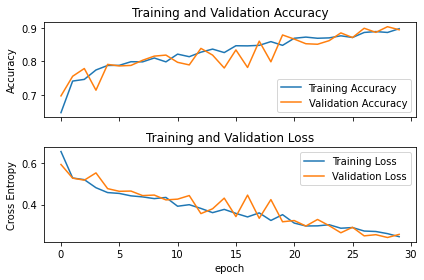
\includegraphics[width=0.4\linewidth]
			{imgs/tf_cnn.png}\label{tf_cnn_cmp}}
			\hspace{0.5cm}
			\subfloat[cnn using fast.ai]
			{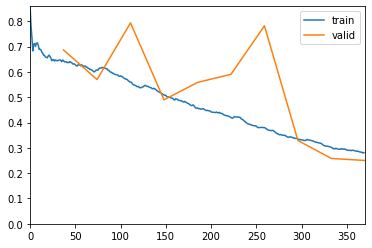
\includegraphics[width=0.5\linewidth]
			{imgs/fastai_cnn.png}\label{fastai_vgg16_cmp}}
			\caption{CNN implemented in fast.ai and tensorflow}
			\label{CNN in fast.ai and tensorflow}
		\end{figure}
	\end{frame}

	\begin{frame}
		\frametitle{Results}
		\framesubtitle{VGG 16 implemented using fast.ai and tensorflow}
		\begin{figure}[H]
			\centering
			\subfloat[vgg16 using tensorflow]
			{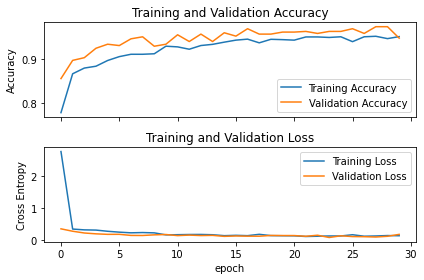
\includegraphics[width=0.4\linewidth]
			{imgs/tf_vgg16.png}\label{tf_vgg16}}
			\hspace{0.5cm}
			\subfloat[vgg16 using fast.ai]
			{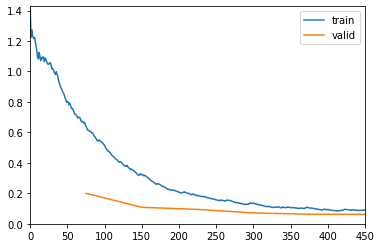
\includegraphics[width=0.5\linewidth]
			{imgs/fastai_vgg16.png}\label{fastai_vgg16}}
			\caption{VGG16 implemented in fast.ai and tensorflow}
			\label{VGG16 in fast.ai and tensorflow}
		\end{figure}
	\end{frame}

	\begin{frame}
		\frametitle{Results}
		\framesubtitle{ResNet 50 implemented using fast.ai and tensorflow}
		\begin{figure}[H]
			\centering
			\subfloat[resnet50 using tensorflow]
			{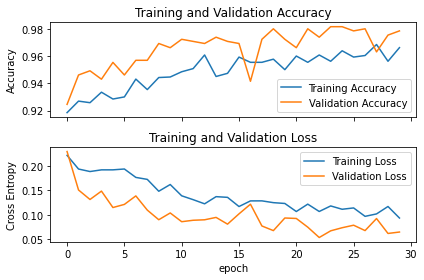
\includegraphics[width=0.4\linewidth]
			{imgs/tf_resnet.png}\label{tf_resnet}}
			\hspace{0.5cm}
			\subfloat[resnet50 using fast.ai]
			{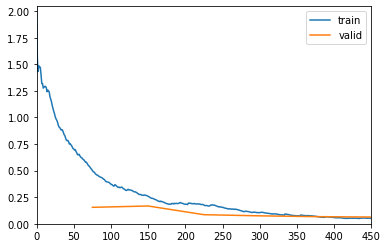
\includegraphics[width=0.5\linewidth]
			{imgs/fastai_resnet.png}\label{fastai_resnet}}
			\caption{Resnet 50 implemented in fast.ai and tensorflow}
			\label{ResNet 50 in fast.ai and tensorflow}
		\end{figure}
	\end{frame}

	\begin{frame}
		\frametitle{Results}
		\framesubtitle{Predictions}

		\begin{figure}[H]
			\centering
			\subfloat[prediction made by VGG16 implemented in tensorflow]
			{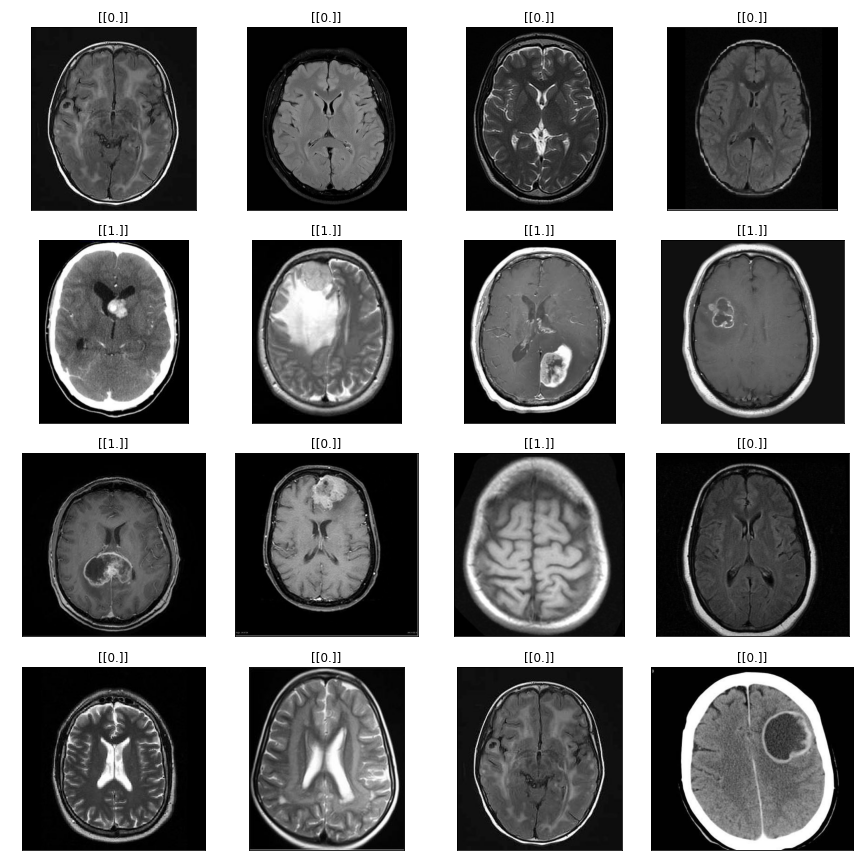
\includegraphics[width=0.3\linewidth]
			{imgs/result.png}\label{vgg16_tf}}
			\hspace{0.3cm}
			\subfloat[prediction made by ResNet50 implemented in fast.ai]
			{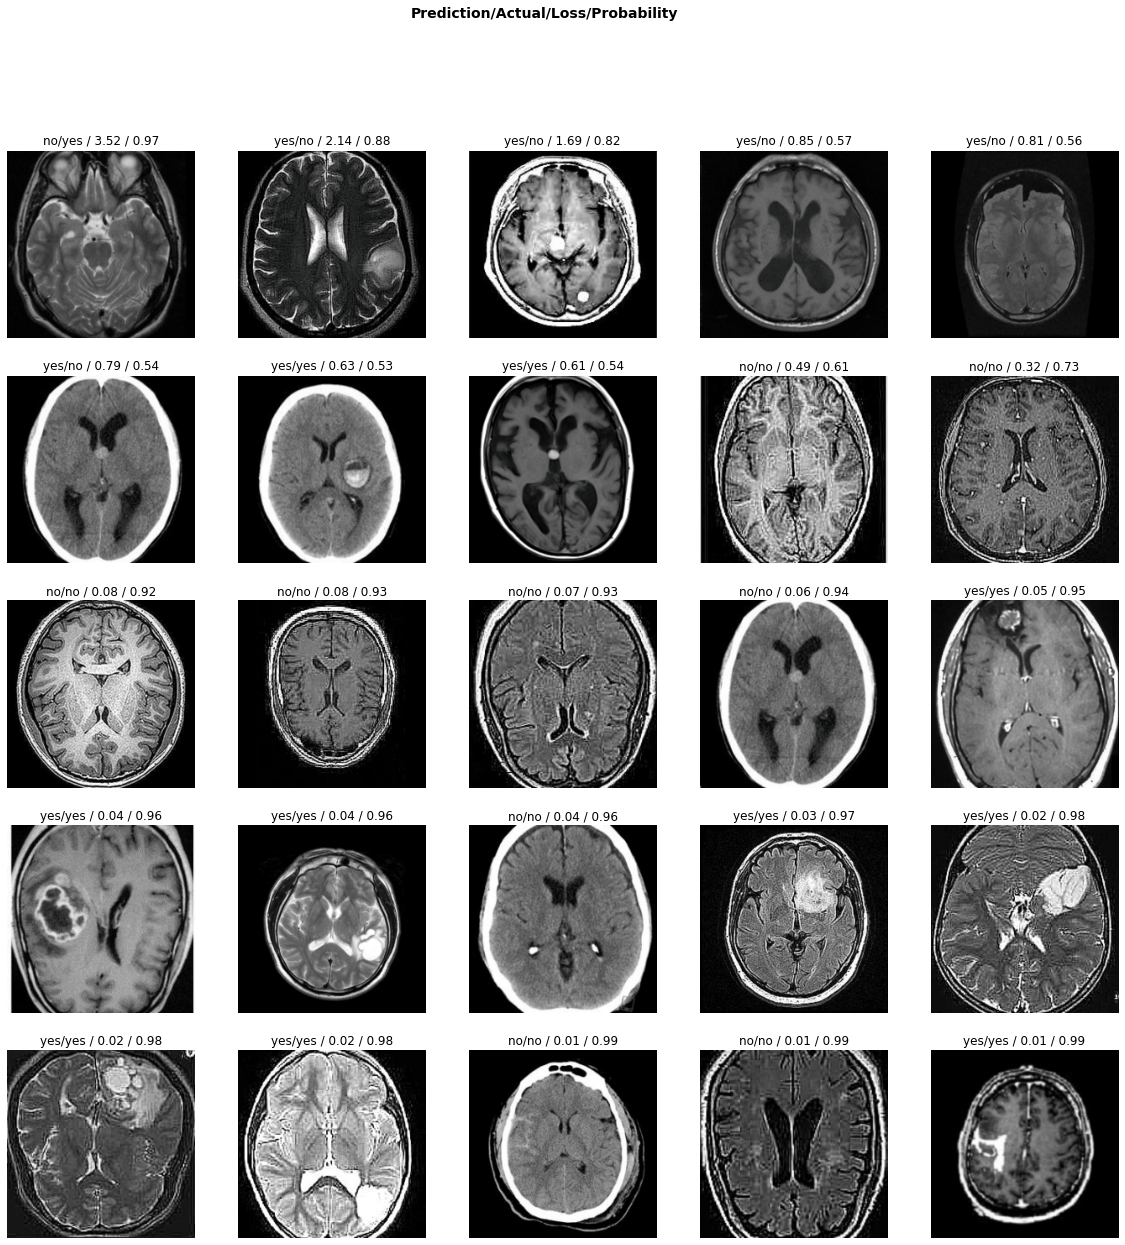
\includegraphics[width=0.3\linewidth]
			{imgs/result_fast_ai.png}\label{resnet_fastai}}
			\caption{Comparing Predictions made by models}
			\label{fig:Results_Comparison}
		\end{figure}
	\end{frame}

	\begin{frame}
		\frametitle{Result}
		\framesubtitle{Comparing the model accuracies}

		\begin{table}
			\begin{center}
				\begin{tabular}{| c | c | c |}
					\hline
					Model & Implementation using TensorFlow & Implementation using
					fast.ai \\
					\hline
					CNN & 90.31\% & 92.66\% \\
					\hline
					VGG 15 & 97.38\% & 98.15\% \\
					\hline
					ResNet 50 & 97.54\% & 99.00\% \\
					\hline
				\end{tabular}
				\caption{Results in percent of the models implemented}
			\end{center}
	\end{table}
	\end{frame}

	\section{Future Work}
	\begin{frame}
		\frametitle{Future Work}

		We further plan on implementing out experiments on other better machine
		learning model such as \textbf{GAN}

		\vspace{0.5cm}

		A generative adversarial network (GAN) is a class of machine learning
		frameworks designed by Ian Goodfellow and his colleagues in 2014. Two
		neural networks contest with each other in a game (in the form of a
		zero-sum game, where one agent's gain is another agent's loss).

		\vspace{0.5cm}

		We also plan on increasing out dataset for better training results.
	\end{frame}

	\begin{frame}
		\centering
		\textbf{\Huge Thank you}
	\end{frame}
\end{document}
